\chapter{ContactPlanの臨時更新の惑星内への限定的な伝播の提案}
\label{chap:suggestion}
本章では、前章でContact Planの臨時更新時に述べた課題に対して、その解決策が満たすべき要件について整理し、
その解決策として、Contact Planの臨時更新の際の情報拡散を惑星内に限定することを提案する。

\section{Contact Planの臨時更新における要件}
ここでは、Contact Planの臨時更新において満たされるべき要件を整理する。
\subsection{要件1: Unplanned Updateによる遅延抑制機能の維持}
ここでは、Contact Planの臨時更新において満たされるべき要件として、
そもそもの目的である実態とかけ離れた状態でCGRを続けることを回避し遅延を抑制すると言う目標にたいして、
情報伝搬範囲を限定することで本提案がそのメリットを損なわないかが重要であるということを述べる。
\subsection{要件2: 他天体にUnplanned Updateをすることによるリソース消費}


\section{臨時更新時に求められる要件と提案手法の対応}

\subsection{要件1に対する提案手法の対応}
\begin{figure}[tbh]
    \centering
    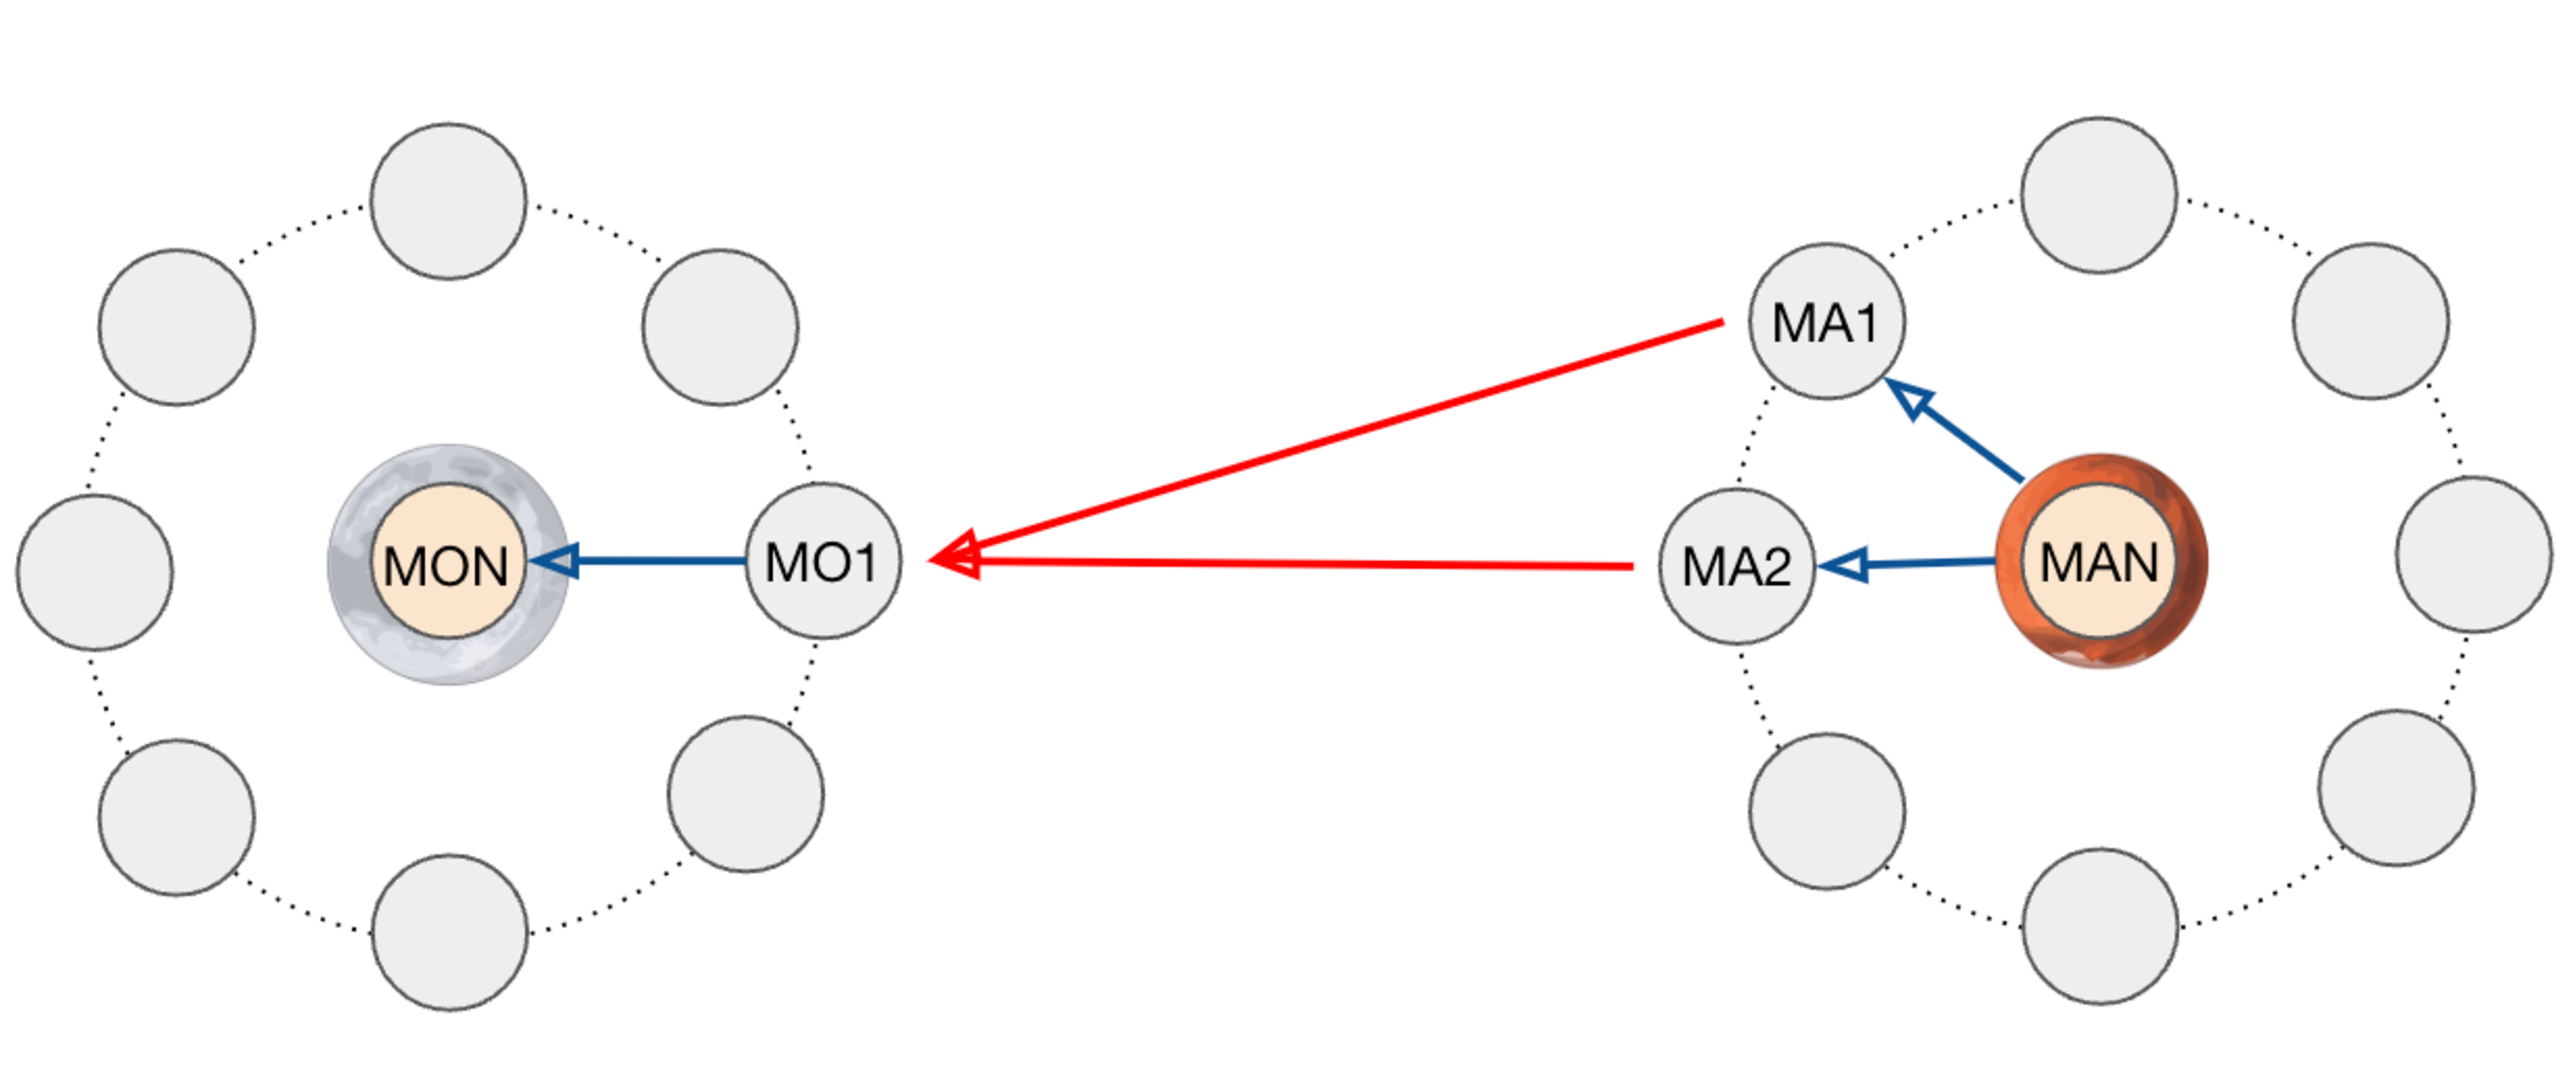
\includegraphics[width=0.7\textheight]{img/ipn_topology.pdf}
    \caption{2040年代以降のIPNのトポロジー}
    \label{fig:dtnprotocolstack}
    \begin{minipage}{\textwidth}
        \raggedright
       2040年代以降、IPNは火星にも拡大し、地球・月・火星の3天体間でのIPNが形成される可能性が想定できる。
    \end{minipage}
\end{figure}

\subsection{要件2に対する提案手法の対応}

\section{Contact PlanのUnplanned Updateの実装}
